\section{An exploratory experiment to illustrate the impact of compute constraints on data choice}
\label{sec:freq}
\begin{figure}[!h]
  \centering
  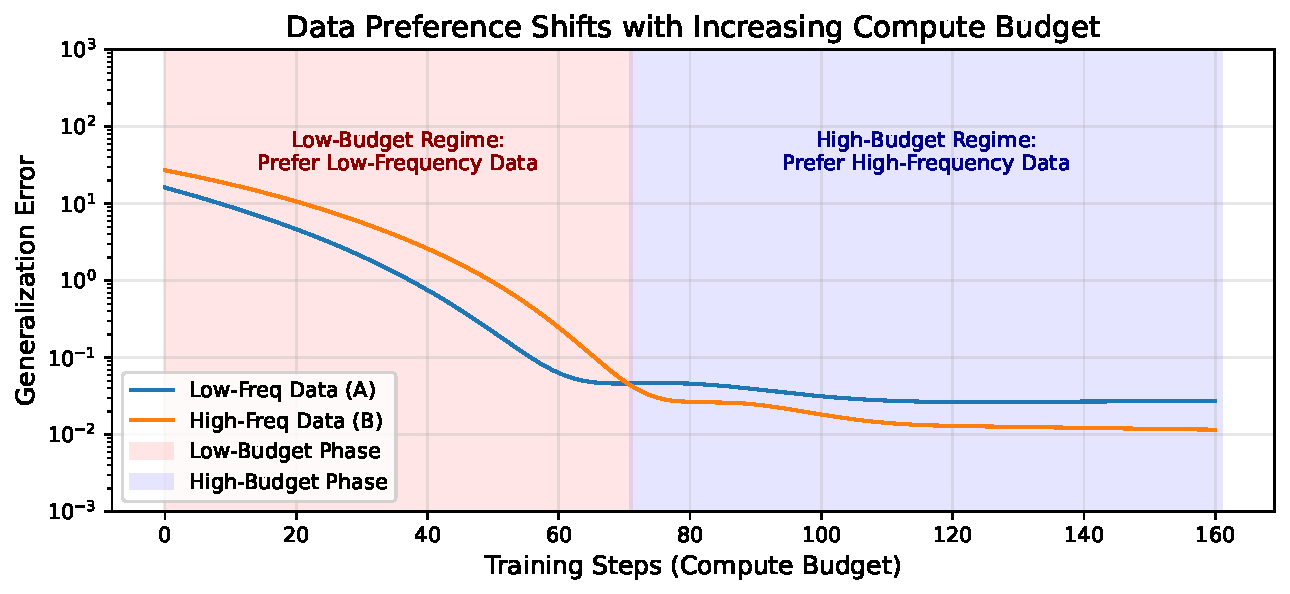
\includegraphics[width=0.7\textwidth]{pics/02_training_dynamics.pdf}
  \caption{Validation loss of models trained on low- and high-frequency data under varying compute budgets. Two regimes emerge: low-budget favors low-frequency data, while high-budget favors high-frequency data, showing compute’s effect on data choice.}
  \label{fig:impact}
\end{figure}

The spectral bias of neural networks—favoring learning low-frequency features before higher-frequency ones—has been well documented in prior work~\cite{Rahaman2018OnTS}. Their findings highlight that models naturally prioritize simpler, low-frequency information early in training. In this section, we build upon this insight to explore the relationship between computational budget and data selection more explicitly. To visualize this connection, we adopt a simple synthetic data generation scheme designed for interpretability.

Specifically, inspired by~\cite{Rahaman2018OnTS}, data are sampled from the function \( y = x + \frac{\sin(\pi x)}{\pi x} \) (where the fraction equals 1 when x = 0) with additive Gaussian noise.  The low-frequency dataset (Model A) samples exclusively at \(\sin(\pi x) = 0\) points, capturing linear patterns. The high-frequency dataset (Model B) samples uniformly across the domain, preserving spectral complexity. Both datasets contain 50,000 samples each to control for size effects, isolating differences to spectral properties alone. We employ a three-layer fully connected network with ReLU activations; architectural details appear in the appendix.
Figure~\ref{fig:impact} presents validation loss trajectories across varying computational budgets. With limited compute, the low-frequency model demonstrates superior generalization. As compute increases, the high-frequency model achieves better performance, confirming the advantage of richer data when resources permit.
These findings establish two distinct regimes in data preference determined by computational constraints, necessitating budget-aware data selection methods that dynamically adapt to available compute—a central focus of this work.
